\pagebreak
\section{Anhang}
\label{sec:anhang}

\begin{figure}
    \centering
    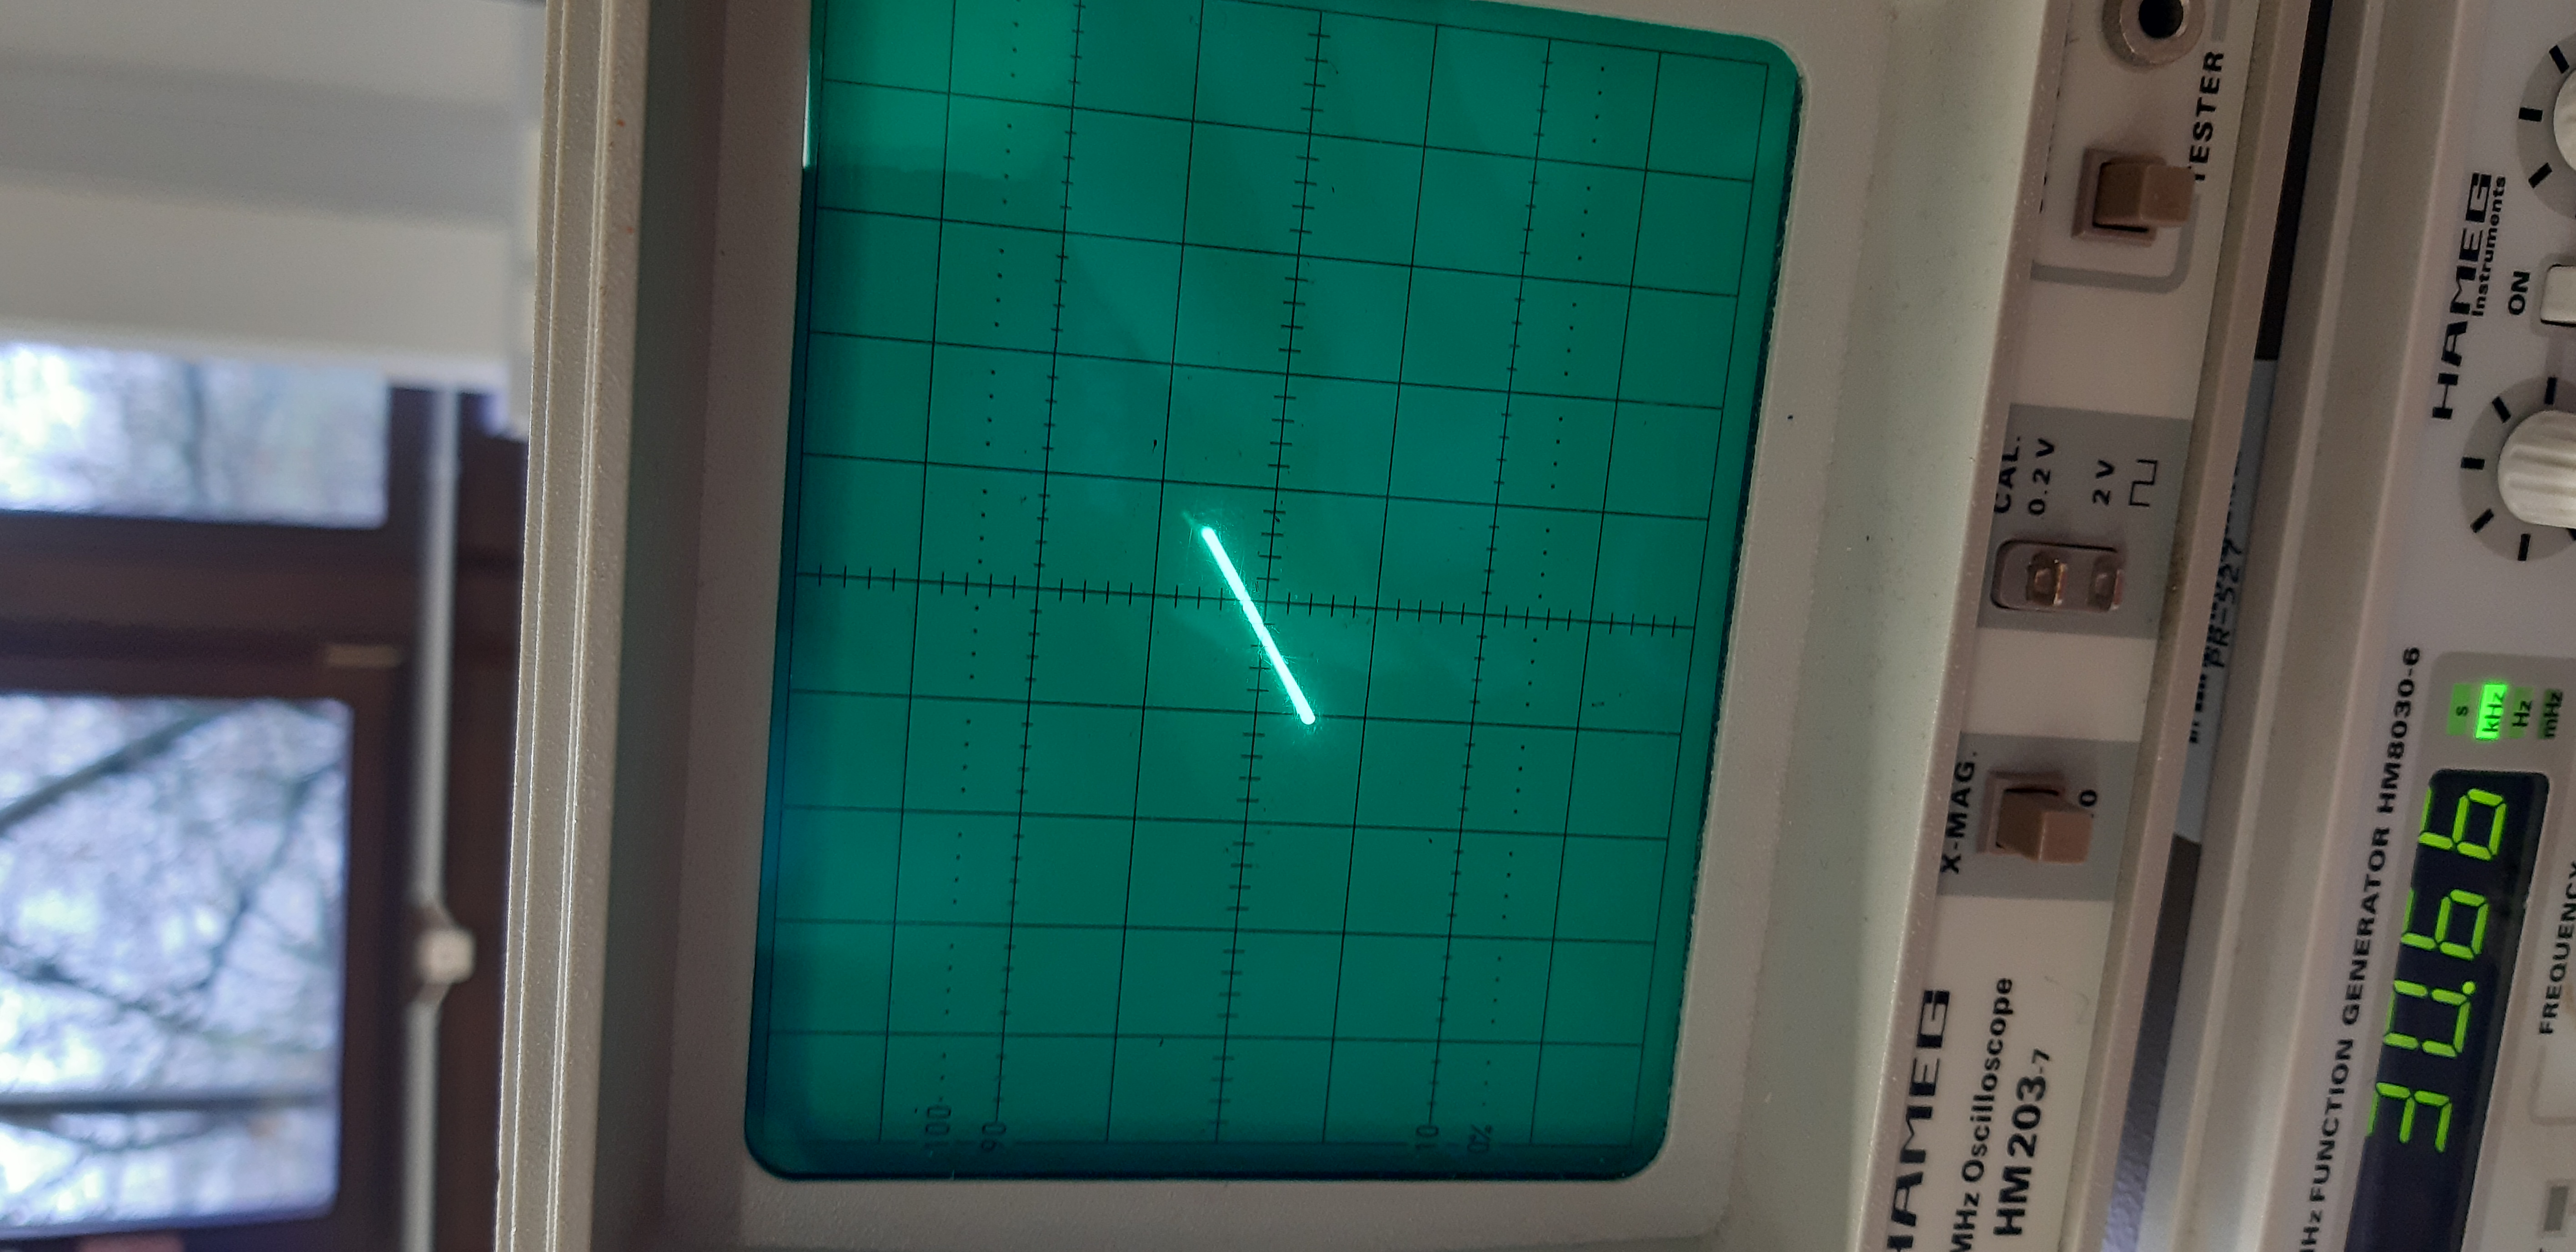
\includegraphics[width=0.75\textwidth, angle=-90]{plots/Lissajour-Gerade.jpeg}
    \caption{Lissajous-Figur der Justierung.}
    \label{fig:Lissajous}
\end{figure}

\begin{figure}
    \centering
    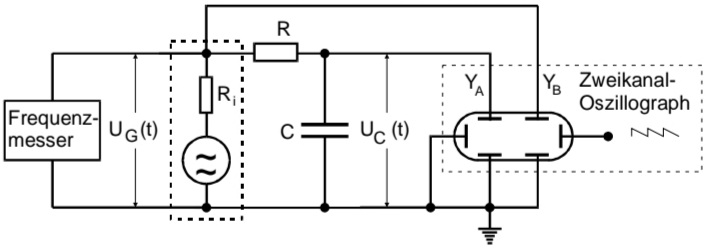
\includegraphics[width=0.75\textwidth]{plots/Schaltung3.png}
    \caption{gekoppelte Schwingkreise \cite{Versuchsanleitung}}
    \label{fig:schaltung3}
\end{figure}


\begin{figure}
    \centering
    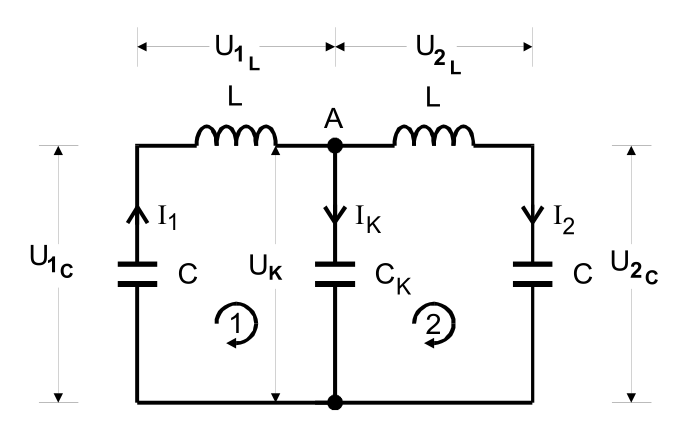
\includegraphics[width=0.75\textwidth]{plots/Schaltung2.png}
    \caption{Schaltung zweier gekoppelter Schwingkreise \cite{Versuchsanleitung}}
    \label{fig:schaltung2}
\end{figure}


\begin{figure}
    \centering
    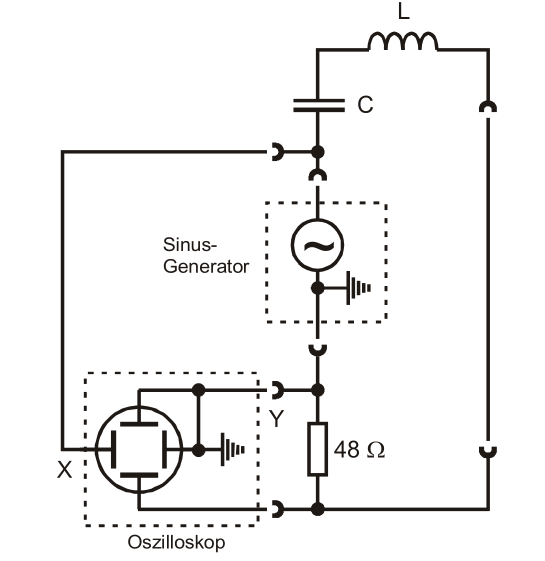
\includegraphics[width=0.75\textwidth]{plots/Schaltung0.png}
    \caption{Schaltung zur Einstellung der Resonanzfrequenz \cite{Versuchsanleitung}}
    \label{fig:schaltung0}
\end{figure}

\begin{figure}
    \centering
    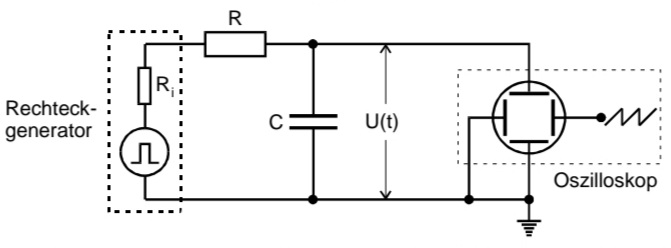
\includegraphics[width=0.75\textwidth]{plots/Schaltung1.png}
    \caption{Schaltung für den Austausch der Schwingungsenergie \cite{Versuchsanleitung}}
    \label{fig:schaltung1}
\end{figure}